\chapter[SCP-068 金属丝小人]{
    SCP-068 The Wire Figure\\
    SCP-068 金属丝小人
}

\label{chap:SCP-068}

\begin{figure}[H]
    \centering
    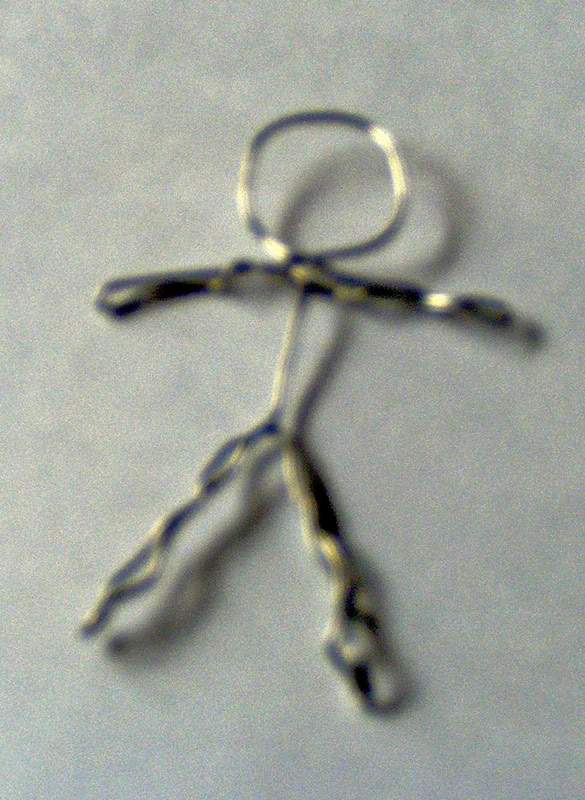
\includegraphics[width=0.4\linewidth]{images/SCP.068.jpg}
    \caption*{SCP-068处于休眠阶段}
\end{figure}

\bb{项目编号:}SCP-068

\bb{项目等级:}Euclid

\bb{特殊收容措施:}SCP-068被保存在一个绝缘的盒子里,盒子的材料最好采用聚四氟乙烯(特氟纶)和橡胶,并远离任何金属。上述的盒子需存放在Site 11的26号保险柜里。钥匙由Wacey博士保管,任何对SCP-068进行测试的申请必须转交给他。

\bb{描述:}SCP-068是一个由一种未知材质的金属丝拉成的小人,高1.8厘米。小人由一根金属丝绕成,金属丝本身在多处被扳弯了若干下。

当电流被引到SCP-068上时,它会变“活”并开始自行移动。SCP-068的“关节”都处在人类相应的关节处。激活后,SCP-068会开始搜寻金属材料,在找到后SCP-068将会扒下一小条金属丝,用来造出一个新的类似于它的小人。新创造的小人会和“原版”一起用剩下的材料造出更新的,随后新小人继续创造新复制品。

当如下两个条件之一被满足时,SCP-068将发展到第二阶段。其一是附近再没有更多的金属来创造一个新的复制体,其二是生成了的小人复制体的数量达到上限102个。当如上任一条件被满足达成时,所有的小人将会聚到一起,试着组成一个尽可能大的人形。当总共有102个“迷你小人”时,他们所汇聚成的大人形会有2米高。SCP-068自己会跑到大人形的躯干和胳膊、头的交点处。在融合完成后,SCP-068会放出γ波、β波和θ波\footnote{\bb{译注:}γ波、β波和θ波均为脑电波。γ波,频率大于35Hz,长期处于该状态下的人会有生命危险;β波,频率为13~35Hz,当精神紧张和情绪激动或亢奋时出现此波,当人从睡梦中惊醒时,原来的慢波节律可立即被该节律所替代;θ波,频率为4~7Hz,成年人在意愿受到挫折和抑郁时以及精神病患者这种波极为显著。但此波为少年(10-17岁)的脑电图中的主要成分。}。之后SCP-068会开始再次寻找金属来试着创造更多的小人,新的小人会和当时的068一样大,但这些新的复制体不会像SCP-068一样发射脑电波。如果此时SCP-068没有到达其规模上限,它将会继续创造更多的复制体,然后把它们融合到自身直到变得最大。

如果SCP-068发展到了第二阶段,且没有足够的金属来造新的小人,SCP-068会在4分32秒的活动后转换到休眠阶段。初始小人周围的一切材料都必须被熔化掉以便重新进行收容。

SCP-068会把所有在它附近的金属造成小人,无论金属的属性。同时,所有尝试损坏、摧毁SCP-068的尝试都失败了。但是,SCP-068的复制体们都拥有和其材料金属同样的属性和弱点。

SCP-068能用一种未知的方式探测到视野外的金属。虽然068不会试着去拿特别难得到的金属,但它会扯开它的四肢能扯开的一切。068的形状不同,它能扯开的最硬的物体也不同。

\bb{附录068-a:}建议使用SCP-068处理危险金属类SCP。

\bb{附录068-b:}\ii{请查看文档068-a}

\bb{文档\#068-a:}\ii{使用SCP-068处理危险金属类SCP的建议被否决。看看我们这有多少无敌的金属SCP,这么做的话我们只可能会眼睁睁地看着一堆干不掉的金属丝小人满Site乱跑。说真的,这主意谁想的?}

\ii{-█████博士}
